
\documentclass[12pt]{article}
\usepackage[utf8x]{inputenc}
\usepackage{amsmath}
\usepackage{graphicx}
\graphicspath{{Images/}}
\usepackage[colorinlistoftodos]{todonotes}
\usepackage{hyperref}

\begin{document}
\begin{titlepage}
\newcommand{\HRule}{\rule{\linewidth}{0.1mm}} 
\center % Center everything on the page
 
\includegraphics[scale=0.3]{iz.jpg}% \\[0.5cm] % 

\textsc{\Large Institut Galilée Université Paris 13 Villetaneuse}\\[0.5cm] % heading course name
\textsc{\large 2018-2019 }\\[0.5cm] % Minor heading


\HRule \\[0.4cm]
{ \huge \bfseries Projet LEE \\
 \large créer un backend permettant de modifier un arbre de décision avec java (Accueil international) }\\[0.1cm]
\HRule \\[1.5cm]


\begin{minipage}{0.4\textwidth}
\begin{flushleft} \large

\emph{Réalisé par :}\\
Chanez \textsc{Chouggar}\\
% Enter Your name and T.No.
\end{flushleft}
\begin{flushleft} \large

\emph{Enseignant:}\\
M. Pierre \textsc{Boudes}\\ 
\end{flushleft}
\end{minipage}
\end{titlepage}


\tableofcontents          % Required
\newpage

% Do not edit the below sections, enter all details in respective chapters
% Add the images/screen-shorts to the image folder and insert them in the respective chapters

\section{Introduction}
\paragraph{}
Les algorithmes d’apprentissage basés sur les arbres sont considérés comme l’une des méthodes d’apprentissage supervisé les plus utilisées. Les méthodes basées sur les arbres donnent aux modèles prédictifs une grande précision, stabilité et facilité d’interprétation. Contrairement aux modèles linéaires, ils mappent assez bien les relations non linéaires. Ils sont adaptables à la résolution de tout type de problème (classification ou régression).
La décision de classification stratégique affecte considérablement la précision d'un arbre. Les critères de décision sont différents pour les arbres de classification et de régression.
Les arbres de décision utilisent plusieurs algorithmes pour décider de diviser un nœud en deux sous-nœuds ou plus. La création de sous-nœuds augmente l'homogénéité des sous-nœuds résultants. En d'autres termes, on peut dire que la pureté du nœud augmente par rapport à la variable cible. L'arbre de décision divise les nœuds de toutes les variables disponibles, puis sélectionne le fractionnement, ce qui donne les sous-nœuds les plus homogènes.

\section{Pourquoi des arbres de décision?}

On opte souvent pour la classification avec les arbres de décision car : 

\begin{enumerate}

\item Les ressources décisionnelles imitent souvent la pensée humaine. Il est donc si simple de comprendre les données et d’interpréter correctement.
\item Les arbres de décision permettent de voir la logique d'interprétation des données (contrairement aux algorithmes de type boîte noire tels que SVM, RN, etc.).

\end{enumerate}

Par exemple:\\
On s’inspire du service de création de feuille de route pour l’arrivée en France des étudiants(es), chercheurs et chercheuses de la Comue Paris Saclay.
Votre arrivée en France? 

\begin{enumerate}

\item Vous vous installez en France pour la première fois
\begin{enumerate}
\item Stagiaire étudiant

\begin{enumerate}
\item EEE ou Suisse
\item autre
\end{enumerate}

\item Doctorant
\end{enumerate}
\item Vous \'etudiez ou travaillez dans un \'etablissement membre et vous  devez renouveler votre titre de séjour
\begin{enumerate}
\item VLS-TS " Etudiant " ou Carte de s\'ejour " Etudiant "
\item Carte de s\'ejour " Passeport talent "
\end{enumerate}

\end{enumerate}

Un arbre de d\ ' ecision est un arbre dans lequel chaque nœud représente une caractéristique (attribut), chaque lien (branche) représente une décision (règle) et chaque feuille représente un résultat (valeur catégorique ou continue).


\section{Algorithme AD}
\paragraph{}
Dans l’implémentation de mon AD, j’ai opté pour un arbre de décision binaire afin d’avoir une visualisation plus compréhensible et interprétable, ce processus sera valable pour les arbres de décisions n-aires.\\Pour l’insertion des nœuds j’ai implémenté un arbre de décision binaire complet ou chaque nœud reçoit deux fils (gauche et droit).  
La recherche se fait en profondeur (pré-ordre, in-ordre et post-ordre) ce qui permet de parcourir l’arbre selon le choix effectué (0 : gauche et 1 : droite).\\
\begin{center}
 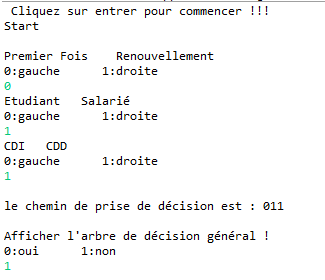
\includegraphics {Images/1.png}% \\[0.5cm] % 
\end{center}
\\Le processus de fonctionnement de cet algorithme est le suivant :
\\Dans un premier temps on crée notre arbre avec des données similaires aux données du site web accueil international des étudiants et chercheurs de la Comue Paris Saclay ; une fois le code est créé, l’utilisateur peut effectuer son choix et prendre une décision selon ce qu’il lui ait proposé et saisir soit 0 pour faire le choix de gauche et 1 pour le choix de droite ; à la fin de l’exécution on obtient le chemin parcouru pendant la prise de décision, ce résultat est utilisé et manipulé dans le projet de réalisation de feuilles de route pour finaliser la partie back-end.
\begin{center}
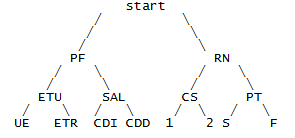
\includegraphics[scale=1]{Images/2.png}% \\[0.5cm] % 
\end{center}

 
\section{Exécution du programme}
Le projet est réalisé sur l’environnement java (eclipse Version: Luna Service Release 2 (4.4.2) Build id: 20150219-0600 JRE  jdk\_8)  

\section{Conclusion}
\paragraph{}
Ce projet a été très bénéfique car il m’a permis de revoir certaines notions d’apprentissage et classification vu dans machine learning, je site le modèle d’apprentissage supervisé, arbres de décision et leur implémentation sous java.

\section{Lien}
https://github.com/ChameeRay/DecisionTreeJava/

\end{document}
